\chapter{Evaluation}
Evaluating an artistic project is difficult as there is a need to separate
aesthetic goals from more technical ones. Testing against the objectives I set
in the introduction may be potentially \emph{subjective} due to the nature of
the project. For example, how can we test if the program ``Allows the user to
experience the works of Viner'', for this some comparison of the methods used in
this project, the possibilities of the images they generate, and the existing
work of Viner needs to be made. User testing is possible to compare against the
user interaction elements, but would not tell the whole story of the more
artistic style.

I have therefore tried to talk about some of the more aesthetic goals and
evaluate them as technically as possible, but with respect to the original
objectives.

\section{User Testing}
The current situation with COVID-19 and meeting people in person made in-person
testing impossible. In my introduction I outlined a use case of an online exhibition
where this work may be displayed; I decided to try and find users online via
social media. This fits the `spirit' of an online exhibition well and allows the
user to explore the program without my influence and without them asking me
questions which should hopefully help reflect on if the program is intuitive to
use, and makes sense generally. Further, my social media `influence' contains a
lot of people who are generally interested in computers, art, and music; so I
feel this is as best of a sample group as possible.

I prepared a questionnaire for completion after the user had been instructed to
play with the program for 5-10 minutes. This included questions on whether it
felt like the user was exploring a landscape, if the audio felt connected to the
graphics, how intuitive the program was to control, how it felt to use the
history function, and two optional free text fields about how it felt to control
the program and a generic 'other' field for capturing any other feelings the
user might have had. I kept the questionnaire short as to encourage a greater
number of responses. The questionnaire is attached \autoref{questionnaire}. In
the end I collected 20 user's responses most of which left text in the free text
fields.

\section{Evaluation}
\subsection{Overall Experience}
Users tended to share a sentiment that the program was slightly confusing at
first but with exploration of the features it began to make sense. One user
said: ``I found it unintuitive at first but I think that was made it engaging at
first. If I felt like I knew how it worked straight away I wouldn't have played
with it for as long. I felt like it was a puzzle.''

This is a good for a program made to engage people, the fact that users were
puzzled but then with some user it began to make sense shows that there is some
learning moment going on; which may cause a feeling of `mastery' over the
program and overall a greater sense of accomplishment than if a full tutorial
was given. This technique is well documented in video games, the most famous
example being World 1-1 of Super Mario Bros for the Nintendo Entertainment
System where concepts are gently introduced without instruction to make the
player feel like they are in control \citep{miyamoto11}.

Another user said that they ``left this open for like 45 mins zoning out to the
noise'' which I think is another sign of overall success and engagement.

\subsection{Reproduction of Viner's Style}
The program cannot reproduce every image that Viner's pen plotter pieces span.
Ultimately this is due to fundamental design decisions in how the program
operates. For example, some of Viner's work includes non-closed polygons the
method outlined in \autoref{Polygons} cannot produce polygons that are not
closed. 

\begin{figure}[H]
    \centering
    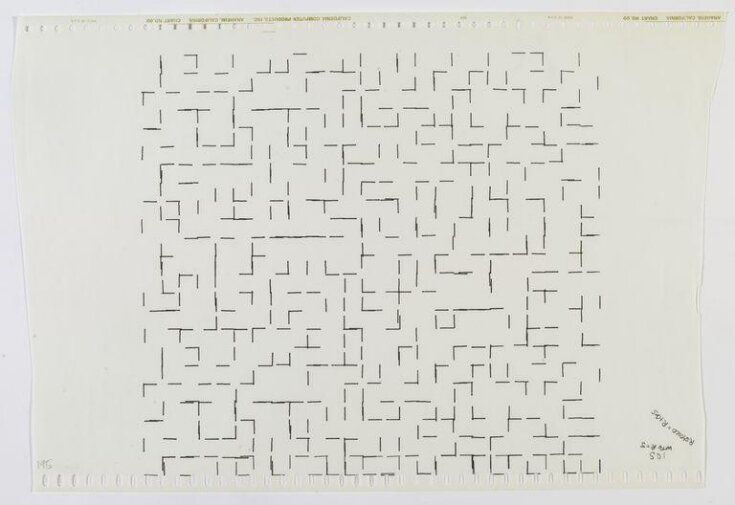
\includegraphics[width=0.7\textwidth]{vinerimpossible}
    \caption{An example of an image that the program cannot reproduce}
\end{figure}

Some of Viner's work contains artefacts from the pen plotter method, which is
also not represented in the final program. This is an example of the medium and
the process he worked with, even if it was not ideal. Perhaps a program that
truly sought to reproduce the totality of his work should reproduce this as
well. Later plotter art by Viner also took on a radically different style, which
isn't explored in this project either.

\begin{figure}[H]
    \centering
    \begin{subfigure}[t]{0.49\textwidth}
        \centering
        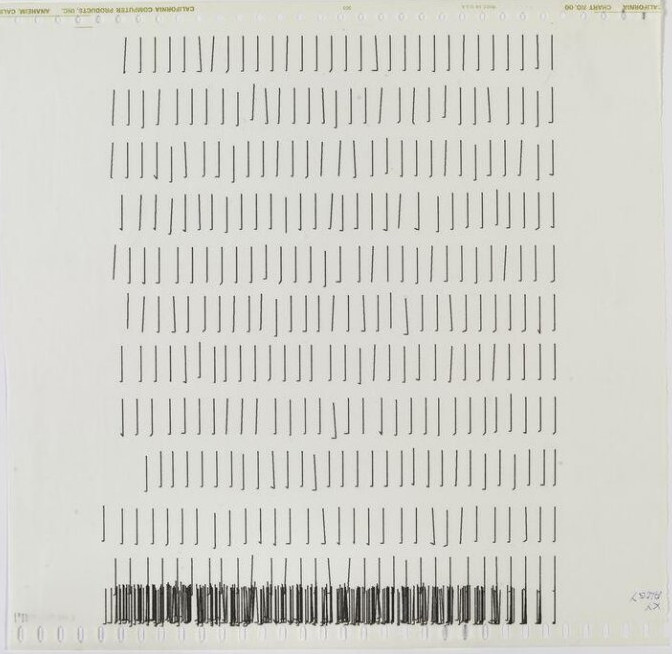
\includegraphics[width=1\textwidth]{vinerbunching}
        \caption{`Bunching' at the bottom of the page, likely due to coordinates
        greater than that of the plotter's maximum range}
    \end{subfigure}
    \hfill
    \begin{subfigure}[t]{0.49\textwidth}
        \centering
        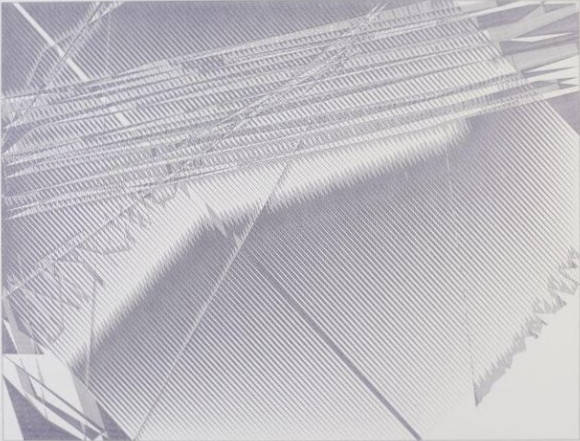
\includegraphics[width=1\textwidth]{laterplotter}
        \caption{An example of Viner's later pen plotter work}
    \end{subfigure}
    \caption{}
\end{figure}

This is not necessarily a failure outright, but does bare mentioning that the
program only explores a subset of Viner's work; which still provides the user
with the sense of exploring a possible `landscape' of which these images are
part of.

Fixing this would require some fundamental reworking to the way the graphics are
generated, perhaps creating the grid as a set of points and finding a way to
work out if the points should be drawn or lines between points should be drawn.

\subsection{Methods Used}
I believe that the methods outlined in \autoref{landgen} and
\autoref{Music} (specifically: \autoref{sonicnav} and
\autoref{Sequencing}) were successful in the sense that they are tools that
could be reused in any project.

The methods for auditory location outlined in \autoref{sonicnav} are of interest
to me to develop further as I believe they could be expanded to work well with
existing data visualisation programs and perhaps be used as a novel way to
explore multi-variate datasets as an extra part of, for example the grand tour
method as in \citep{asimov1985grand}; a chord could play with the intervals
marking the subsets you are viewing and move between chords as the image on the
screen changes. More exploration could also be completed with rhythm which is a
good use of temporal data, perhaps using `beats' as marks on a `ruler' in space
you are travelling through in time, with acceleration these beats get closer
together.

The noise `approximate rounding' method in \autoref{landgen} is an example of a
technique that can be fully integrated into another project at will, this was
successful example of creating a technique that is applicable to other projects
that utilise point-wise noise.

\subsection{User Interface}
Some users in testing pointed out that the help menu would be cut off on smaller
screens (e.g. older laptops) so I implemented some responsive CSS using
\verb|@media| queries to allow for it to be used on smaller screens. I did this
during user testing as I believe it was important to the user's experience of
other elements of the program for the purposes of evaluation. Similarly, an
issue with some elements (the volume slider and mute button) not repositioning
themselves if the screen resized. I also fixed this during user testing.

One user commented that they used an AZERTY keyboard which this program does not
support so they had to switch to QWERTY. Whilst not a problem for a physical
exhibition allowing for international or alternative keyboard layouts should be
considered before making this part of an online exhibition.

\subsection{Navigation}
80\% of users felt that they were in a `landscape'. A few interesting comments
about how it felt to control the program were:

\begin{displayquote}
``Once I decided to ignore the descriptions of the controls, and sought to come
up with my own names for them, it began to be intuitive. The discovery of the
landscape-nature was quite interesting, and the experience was overall
enjoyable.''
\end{displayquote}

\begin{displayquote}
``It was simple and rewarding to explore the landscape.''
\end{displayquote}

\begin{displayquote}
``The layout of the keys was a little confusing to me, and it wasn't clear why
some squares moved but not others -- even when I turned the randomness down,
they seemed to still move randomly but more slowly.''
\end{displayquote}

Some users agreed that the image changed too slowly, perhaps the idea of
acceleration as you hold down a button could be introduced to allow people to
move around faster.

\subsection{Audio}
From an artistic perspective I think that the musical aspect was a success, this
is hard to evaluate as it is totally disconnected from even Viner's work.
Ideally I would have included some more depth. I had looked into using various
field recordings from around Leeds I have made as backing for the music but the
technical aspects of this made it impossible to implement without using a
web server meaning the whole application was less portable.

\begin{figure}[H]
    \centering
    \includegraphics[width=0.5\textwidth]{fieldrecording}
    \caption{Field recording setup}
\end{figure}

The majority of users thought that the audio was connected to the graphics but
35\% did not. Perhaps a more explicit explanation or some change to make it more
immediately obvious to the user could help. Recalling \autoref{Composition} one
user said that the music reminded them of ``90s Brian Eno quite a bit''.

A few users commented that the audio did not sound at all, it seemed to be
mostly Google Chrome users. This would require extra testing before deployment
to a remote gallery but, again, might not be a problem on a single installation
where only one computer is used.

\subsection{History}
Users generally understood the history function, only 10\% said that it did not
function as expected. For some users the tree ended up going off screen; to fix
this more work would need to be done to create a method to scroll up and down
it.

One user suggested that there should be the ability ``[...] to decide when a
node on the tree was created, rather than have this happen automatically.''
Which is an interesting idea, perhaps two modes could be provided `automatic'
and `manual' with a button to add a new node at will, or maybe a different
colour colour be used for manually saved states. This would allow users to fully
save and recall states that they wish to revisit.

Some users commented that they found the upload and download confusing, and that
perhaps I should limit the possible uploaded files to only the
`application/json' MIME type so as to not let the user think any arbitrary file
is uploaded. Also, being in a web browser the user might think that the
uploaded files are stored on an external server which is not the case; The file
never leaves their computer. Some method to let the users know this is the case
would be helpful
